% ══════════════════════════════════════════════════════════════════
%  Tesis Doctoral — formato UPS (basado en la plantilla tesis.tex)
%  "Modelo de Gobernanza Legaltech Adaptativa basada en Inteligencia
%   Artificial para Flujos Procesales jurídicos" (MALTG)
%  Compilar: pdflatex → bibtex → pdflatex ×2
% ══════════════════════════════════════════════════════════════════
\documentclass[a4paper,openany,12pt]{book}

\usepackage[utf8]{inputenc}
\usepackage{savetrees}
\usepackage[hidelinks]{hyperref}
\usepackage{times}
\usepackage{amsfonts}
\usepackage{amsmath}
\usepackage{multirow, array}
\usepackage{graphicx}
\usepackage{float}
\usepackage[spanish,es-tabla]{babel}
\usepackage[flushleft]{threeparttable}
\selectlanguage{spanish}
\usepackage[spanish,Algoritmo]{algorithm}
\usepackage{afterpage}
\usepackage{vmargin}
\usepackage[table,xcdraw]{xcolor}
\usepackage{rotating}
\usepackage[font={footnotesize,it}]{caption}
\usepackage{fancyhdr}
\usepackage{algorithmic}
\usepackage{subfigure}
\usepackage{titlesec}
\usepackage{booktabs}

\title{Modelo de Gobernanza Legaltech Adaptativa basada en Inteligencia Artificial para Flujos Procesales jurídicos}
\author{Nombre1 Nombre2 Apellido1 Apellido2}
\setcounter{secnumdepth}{5}
\setcounter{tocdepth}{5}
\renewcommand{\baselinestretch}{1.5}

\setmargins{3.5cm}{1.5cm}{14cm}{23.42cm}{10pt}{1cm}{0pt}{2cm}
\titleformat{\chapter}[block]{\normalfont\huge\bfseries}{\chaptertitlename\ \thechapter}{20pt}{\Huge}

\begin{document}
% ═══ PORTADA ═══
\begin{titlepage}
\begin{center}
\vspace*{-1in}
\begin{figure}[htb]\begin{center}
\includegraphics[width=8cm]{escudoUPS}\end{center}\end{figure}
\begin{large}
\vspace{0.15cm}\textbf{UNIVERSIDAD POLITÉCNICA SALESIANA}\\
\vspace{0.5cm}\textbf{SEDE MATRIZ CUENCA}\\
\vspace{0.5cm}\textbf{Doctorado en Ciencias Computacionales}\\
\vspace{0.75cm}\textbf{Tesis Doctoral}\\ \vspace{0.75cm}
\end{large}
\begin{large}
\textbf{Título:}\\Modelo de Gobernanza Legaltech Adaptativa\\basada en Inteligencia Artificial\\para Flujos Procesales jurídicos\\
\vspace{0.75cm}\textbf{Autor:}\\Nombre1 Nombre2 Apellido1 Apellido2\\
\vspace{0.75cm}\textbf{Director:} Dr. Nombre1 Nombre2 Apellido1 Apellido2\\
\textbf{Co-Tutor:} Dr. Nombre1 Nombre2 Apellido1 Apellido2\\
\vspace{1.5cm}\textbf{Fecha:} Julio 2026\\
\end{large}
\end{center}
\end{titlepage}
\afterpage{\null\newpage}
\thispagestyle{empty}\newpage
\chapter*{}
\frontmatter

\begin{flushright}\textit{Dedicado a \ldots \vspace*{2cm}\\ }\end{flushright}
\afterpage{\null\newpage}
\cleardoublepage

\chapter*{}
\section*{Declaración de autoría}
Yo, Nombre1 Nombre2 Apellido1 Apellido2, declaro que esta tesis titulada ``Modelo de Gobernanza Legaltech Adaptativa basada en Inteligencia Artificial para Flujos Procesales jurídicos'' y el trabajo presentado en ella es de mi autoría, conforme a las condiciones de originalidad y atribución establecidas por la Universidad.
\cleardoublepage

\chapter*{Agradecimientos}
A \ldots
\cleardoublepage

\section*{Resumen}
La administración de justicia ecuatoriana dispone, con el Código Orgánico General de Procesos (COGEP), de términos procesales taxativos cuyo incumplimiento es sancionable (Art.~93); sin embargo, la gobernanza tecnológica del ecosistema judicial carece de mecanismos que midan ese cumplimiento de forma continua y retroalimenten la toma de decisiones. Esta tesis diseña, construye y evalúa ---bajo la metodología \textit{Design Science Research} (DSR)~\cite{hevner2004,peffers2007}--- el modelo MALTG: (i) una ontología multicapa de gobernanza (TOGAF, COBIT, ITIL, NIST, dominio legaltech) formalizada en OWL; (ii) un \textit{structural digital model} del ecosistema tecnológico del Consejo de la Judicatura, construido mediante análisis documental sistemático con evidencia SHA-256; (iii) una \textit{cognitive digital shadow} que razona simbólicamente sobre expedientes reales del sistema e-SATJE aplicando las reglas de término del COGEP; y (iv) un ciclo adaptativo \textit{MAPE-K} que recalibra los indicadores de gobernanza desde la realidad procesal, gestiona el cambio normativo con aplicación temporal de la norma y emplea las ontologías como \textit{guardrails} anti-alucinación. La evaluación sobre 47 causas reales (60 términos evaluables) arroja un índice empírico global de cumplimiento de 36.7/100 frente a una madurez declarada de 73.9/100; el instrumento de validez del razonador (F1 macro, matriz de confusión, $\kappa$ de Cohen) se demuestra extremo a extremo con una sesión simulada reproducible (semilla 42), y el análisis de sensibilidad muestra estabilidad del modelo ante perturbaciones de $\pm$10\% en los pesos (desviación máxima 0.5 puntos). La contribución principal es un artefacto DSR reproducible que convierte la gobernanza legaltech de un ejercicio declarativo en un sistema de medición adaptativo con trazabilidad criptográfica.

\textbf{Palabras clave:} gobernanza adaptativa, legaltech, design science research, digital twin, ontologías legales, razonamiento simbólico, process drift, COGEP.
\cleardoublepage

\section*{Abstract}
Ecuador's procedural code (COGEP) establishes mandatory procedural terms whose breach is legally sanctionable, yet the technological governance of the judicial ecosystem lacks mechanisms to continuously measure compliance. Following Design Science Research, this thesis designs, builds and evaluates MALTG: a multilayer governance ontology (OWL), a structural digital model of the Judiciary Council's technological ecosystem built from hash-verified documentary evidence, a cognitive digital shadow that symbolically reasons over real e-SATJE case files, and a MAPE-K adaptive loop that recalibrates governance indicators from procedural reality, manages regulatory change with temporal application of norms, and uses ontologies as anti-hallucination guardrails. Evaluation over 47 real cases (60 evaluable terms) yields a global empirical compliance index of 36.7/100 against a declared maturity of 73.9/100; the reasoner validity instrument (macro F1, confusion matrix, Cohen's $\kappa$) is demonstrated end-to-end with a reproducible simulated session (seed 42), and sensitivity analysis shows model stability under $\pm$10\% weight perturbations (max deviation 0.5 points). The main contribution is a reproducible DSR artifact that turns legaltech governance from a declarative exercise into an adaptive measurement system with cryptographic traceability.
\cleardoublepage

\tableofcontents
\listoffigures
\listoftables
\listofalgorithms
\mainmatter

% ══════════════════════ CAPÍTULO 1 ══════════════════════
\chapter{Introducción}
La transformación digital de la justicia ha producido sistemas de expediente electrónico ---en Ecuador, el e-SATJE del Consejo de la Judicatura--- que registran cada actuación procesal con fecha, tipo y responsable. Esa telemetría, sin embargo, se usa casi exclusivamente para consulta: no alimenta la gobernanza tecnológica de la institución ni permite verificar de forma continua el cumplimiento de los términos que el COGEP impone bajo sanción. Simultáneamente, los marcos de gobernanza de TI (TOGAF, COBIT, ITIL, NIST CSF) se evalúan mediante autodeclaraciones de madurez desacopladas del desempeño real del proceso judicial. Esta tesis aborda ese doble desacoplamiento con un artefacto que une ambos mundos mediante un ciclo adaptativo gobernado por ontologías.

\section{Planteamiento del problema}
El problema se descompone en cuatro déficits observables: \textbf{(D1)} los modelos de gobernanza legaltech son estáticos: sus indicadores se declaran, no se miden, y no reaccionan ante cambios en datos, norma o contexto~\cite{janssen2016}; \textbf{(D2)} la variabilidad del contexto fáctico ---las actuaciones reales de los jueces--- y la \textit{process drift} dilatoria no se detectan sistemáticamente~\cite{aalst2012,bose2014}; \textbf{(D3)} la IA aplicada al dominio jurídico enfrenta el riesgo de alucinación, inadmisible donde cada afirmación exige fundamento normativo~\cite{garcez2023,governatori2022}; \textbf{(D4)} el cambio normativo altera las reglas de cómputo, pero los sistemas no versionan el conocimiento jurídico ni aplican la norma vigente a la fecha de cada acto.

\section{Preguntas de investigación e hipótesis}
\begin{table}[H]\centering\footnotesize
\caption{Preguntas de investigación e hipótesis.}\label{tab:rq}
\begin{tabular}{p{0.7cm}p{6.2cm}p{6.2cm}}\toprule
\textbf{ID} & \textbf{Pregunta de investigación} & \textbf{Hipótesis} \\ \midrule
RQ1 & ¿Puede un modelo de gobernanza legaltech recalibrar sus indicadores desde la medición empírica del cumplimiento procesal? & H1: un ciclo MAPE-K que consuma expedientes reales produce indicadores que difieren de los declarados y son trazables a evidencia verificable. \\
RQ2 & ¿Puede un razonador simbólico acotado por una ontología procesal emitir dictámenes con validez medible y sin alucinaciones? & H2: el mapeo providencia$\to$acto es medible contra \textit{gold standard} (F1) y toda salida fuera del vocabulario se rechaza, no se inventa. \\
RQ3 & ¿Es posible detectar dilación (\textit{process drift}) y variabilidad fáctica desde las trazas del expediente, con criterio normativo primario? & H3: los detectores identifican causas atípicas con ranking estable ante perturbaciones $\pm$20\% de los pesos. \\
RQ4 & ¿Puede la adaptación mantenerse trazable y reproducible? & H4: metadatos de contexto (hashes) y bitácora \textit{hash-chained} permiten reproducir cualquier resultado histórico. \\ \bottomrule
\end{tabular}\end{table}

\section{Objetivos de la investigación}
\subsection{Objetivo general}
Diseñar, construir y evaluar, mediante \textit{Design Science Research}, un modelo de gobernanza legaltech adaptativa basada en inteligencia artificial que mida el cumplimiento de los flujos procesales del COGEP sobre expedientes reales y recalibre continuamente los indicadores de gobernanza tecnológica del ecosistema judicial, con garantías de explicabilidad, no-alucinación y trazabilidad.
\subsection{Objetivos específicos}
\textbf{OE1} Formalizar la ontología multicapa MALTG y la ontología procesal COGEP (Procedimiento$\to$Etapa$\to$Acto$\to$Término$\to$Sujeto), verificables con estándares de ingeniería ontológica~\cite{poveda2014,suarez2015}. \textbf{OE2} Construir el \textit{structural digital model} del ecosistema del Consejo de la Judicatura con protocolo documental reproducible y evidencia SHA-256. \textbf{OE3} Implementar la \textit{cognitive digital shadow}: razonador simbólico determinista con calendario judicial configurable (Arts.~73/77 COGEP). \textbf{OE4} Diseñar el ciclo adaptativo MAPE-K: índice empírico, detectores IVF/IDP, gestión del cambio normativo con aplicación temporal, y panel de supuestos con límites mín--máx. \textbf{OE5} Evaluar con \textit{gold standard} (F1, $\kappa$), ponderación experta (AHP/Delphi, CR, $\rho$ de Spearman) y análisis de sensibilidad.

\section{Contribuciones de la tesis}
Según la clasificación DSR de Gregor y Hevner~\cite{gregor2013}: \textbf{(C1)} artefacto de nivel 2: el sistema MALTG operativo (13 módulos, $\sim$65 \textit{endpoints}, contenedor Docker); \textbf{(C2)} teoría de diseño incipiente: el patrón \emph{gobernanza adaptativa gobernada por ontologías} (MAPE-K cuyo \textit{Knowledge} es una ontología legal que actúa como vocabulario de medición y \textit{guardrail}); \textbf{(C3)} instrumentos de medición reutilizables (IVF, IDP, índice empírico, protocolo SHA-256, bitácora \textit{hash-chained}); \textbf{(C4)} primer \textit{dataset} estructurado de cumplimiento de términos COGEP sobre causas públicas del e-SATJE con diseño muestral declarado.

\section{Publicaciones previas y lineamientos de la tesis}
Esta tesis no parte de cero: es la culminación de una trayectoria de investigación publicada por el autor que estableció, de forma incremental y arbitrada, los lineamientos sobre los que se construye el artefacto. La Tabla~\ref{tab:pubs} resume las cinco publicaciones y su papel como fundamento; las Figuras~\ref{fig:pubarq} y~\ref{fig:pubfound} reproducen los lineamientos arquitectónicos publicados que el artefacto instancia.

\begin{table}[H]\centering\footnotesize
\caption{Publicaciones previas del autor que fundamentan la tesis y lineamiento que aporta cada una.}\label{tab:pubs}
\begin{tabular}{p{0.7cm}p{5.2cm}p{3.4cm}p{4.0cm}}\toprule
\textbf{ID} & \textbf{Publicación (venue)} & \textbf{Aporte publicado} & \textbf{Lineamiento en la tesis} \\ \midrule
P1 & \textit{LegalTech Governance in Ecuador: A Systematic Review of the Digital Transformation of Justice} (IEEE)~\cite{paccha2025slr} & SLR con enfoque secuencial-convergente M3S (SLR+SLM+bibliometría), 2008--2025; identifica la ausencia de un modelo integral que articule dimensiones constitucional, legal, institucional y tecnológica & Justificación empírica del problema (D1--D4) y de las brechas B1--B5 del Cap.~2; delimitación del contexto ecuatoriano \\
P2 & \textit{Architecture for LegalTech Governance: A Holistic Multidimensional Framework Integrating AI, Blockchain, Cybersecurity, Workflows and Enterprise Standards} (COLIM 2026)~\cite{paccha2026colim} & Arquitectura de referencia multidimensional que integra COBIT, TOGAF, ITIL, NIST CSF con IA, blockchain y flujos de trabajo en capas estratégica/gobernanza/operativa & Estructura de capas y dimensiones del modelo MALTG (A1) y del radar de validación (Fig.~\ref{fig:pubarq}) \\
P3 & \textit{From Silos to Synergy: A Foundation Layer Architecture for LegalTech Governance} (IEEE)~\cite{paccha2026silos} & \textit{Foundation Layer} que resuelve el déficit estructural de gobernanza de los marcos aislados (silos) mediante una capa de fundamentos común & Capa de fundamentos del SDT y criterio de integración inter-marcos (Fig.~\ref{fig:pubfound}) \\
P4 & \textit{Verifiable Semantic Governance and Algorithmic Transparency: An Ontological Approach to MALTG} (IEEE ETCM 2026)~\cite{paccha2026etcm} & Ontología OWL/RDF MALTG (54 clases, 15 \textit{object properties}, $\sim$500 tripletas); \textit{Bimodal Audit Method} (BAM) y \textit{Global Transparency Index} (GTI=80.89; TOGAF 91.7, LegalTech 69.1) & Ontología de gobernanza del artefacto (A1) y antecedente directo de la auditoría bimodal que el ciclo adaptativo generaliza \\
P5 & \textit{Structural Digital Twin-Driven Conformance Assessment of a LegalTech Governance Ontology: A Reproducible Proof of Concept} (\textit{Information}, MDPI)~\cite{paccha2026info} & Marco formal reproducible: ontología OWL~2 + SDT JSON-LD (39 microservicios, 54 conexiones), \textit{semantic conformance mapping}, función de cobertura jerárquica y métrica de brecha de conformidad sobre 9 dimensiones & Función $\Psi$ de cobertura (Ec.~4.1), métrica de \textit{gap}, formato JSON-LD del SDT y el principio de prueba de concepto reproducible que esta tesis extiende al ciclo adaptativo \\ \bottomrule
\end{tabular}\end{table}

\begin{figure}[H]\centering
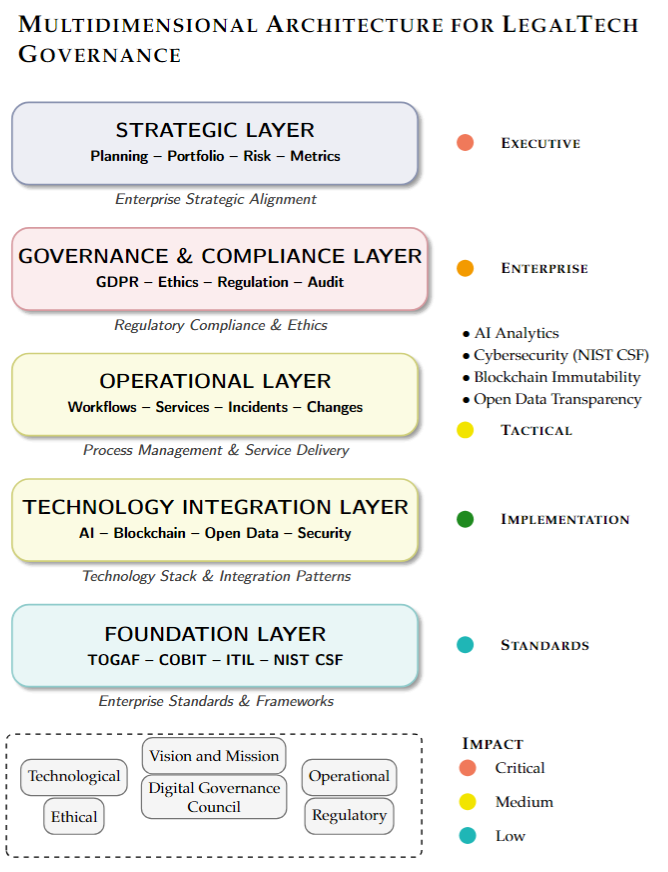
\includegraphics[width=0.9\textwidth]{Figuras/fig_pub_arquitectura}
\caption{Lineamiento publicado (P2): arquitectura multidimensional de gobernanza legaltech que el artefacto instancia como ontología MALTG y radar de validación. Fuente:~\cite{paccha2026colim}.}\label{fig:pubarq}
\end{figure}
\begin{figure}[H]\centering
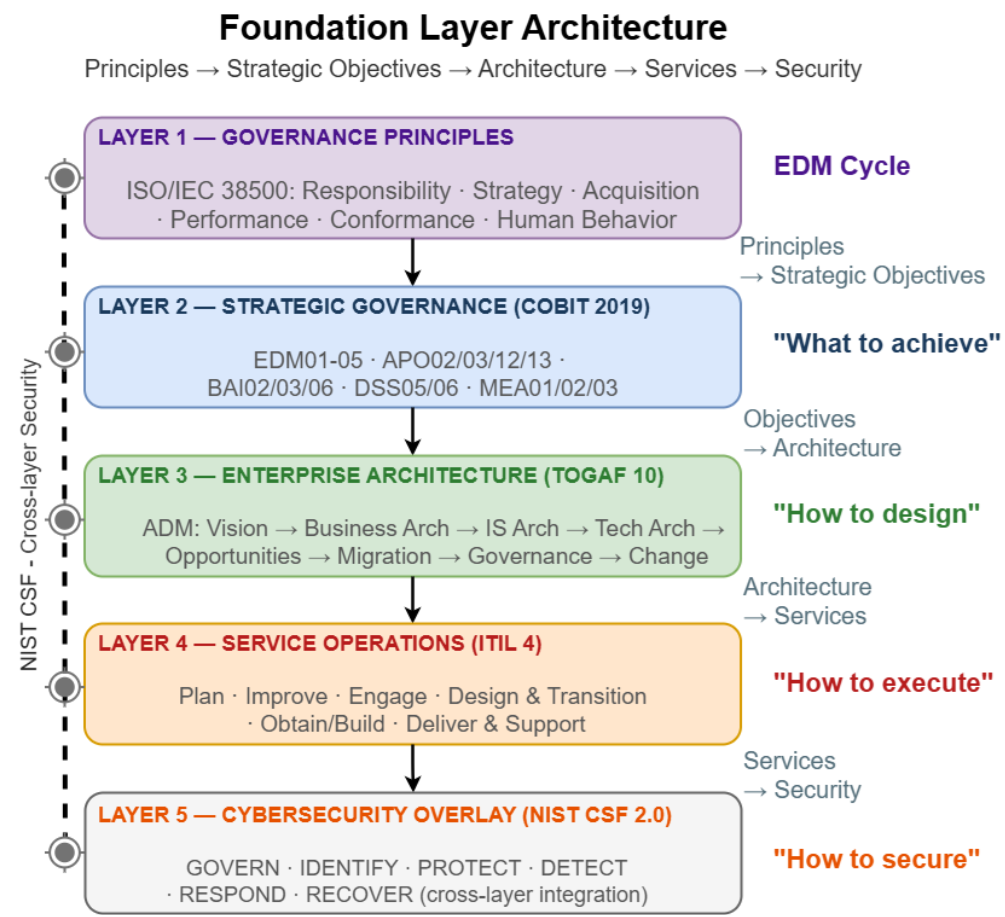
\includegraphics[width=0.9\textwidth]{Figuras/fig_pub_foundation}
\caption{Lineamiento publicado (P3): \textit{Foundation Layer} que integra los marcos de gobernanza en una capa común, base del SDT del artefacto. Fuente:~\cite{paccha2026silos}.}\label{fig:pubfound}
\end{figure}

La progresión es deliberada: P1 establece el \emph{problema} (no existe gobernanza legaltech integral en Ecuador); P2 y P3 publican la \emph{arquitectura} (dimensiones y capa de fundamentos); P4 la \emph{formaliza ontológicamente} y le añade auditoría de transparencia; P5 la hace \emph{medible y reproducible} (SDT + conformidad + $\Psi$). La tesis aporta el eslabón restante: convertir ese aparato estático de conformidad en un \textbf{sistema adaptativo} que se recalibra desde la realidad procesal (MAPE-K), gestiona el cambio normativo y garantiza no-alucinación --- el tránsito de la \emph{conformance assessment} puntual de P5 a la \emph{gobernanza adaptativa} continua.

\section{Alcance y limitaciones}
El alcance cubre procedimientos civiles COGEP sobre causas públicas del portal SATJE (2022--2024). El artefacto es una \textit{digital shadow} (sin retroalimentación al sistema real, condición del \textit{digital twin} pleno~\cite{kritzinger2018}). La muestra (N=47) es intencional estratificada: habilita generalización analítica, no inferencia poblacional. El razonador es simbólico-léxico; su validez se mide contra \textit{gold standard} y se reporta con transparencia permanente en la interfaz.

\section{Estructura del documento}
El Capítulo 2 revisa el estado del arte y sus brechas; el Capítulo 3 formaliza el diseño DSR; el Capítulo 4 presenta el artefacto y la experimentación E1--E5; el Capítulo 5 concluye y proyecta el trabajo futuro.

% ══════════════════════ CAPÍTULO 2 ══════════════════════
\chapter{Estado del Arte}
Este capítulo se apoya en la revisión sistemática publicada por el autor~\cite{paccha2025slr}, que aplicó el enfoque secuencial-convergente M3S (revisión sistemática + mapeo sistemático + análisis bibliométrico) sobre la producción 2008--2025 relativa a la gobernanza legaltech ecuatoriana, y la extiende con las literaturas internacionales de gobernanza adaptativa, gemelos digitales, ontologías legales e IA jurídica.
\section{Fundamentos conceptuales y teóricos}
\textbf{Gobernanza adaptativa.} Janssen y van der Voort~\cite{janssen2016} caracterizan la \textit{adaptive governance} como la capacidad institucional de responder a entornos cambiantes manteniendo estabilidad y rendición de cuentas. El referente computacional es la \textit{autonomic computing}~\cite{kephart2003} y su patrón MAPE-K, que esta tesis traslada a la gobernanza legaltech haciendo del \textit{Knowledge} una ontología jurídica.
\textbf{Gemelos digitales.} La taxonomía de Kritzinger et al.~\cite{kritzinger2018} distingue \textit{digital model}, \textit{digital shadow} y \textit{digital twin}; Tao et al.~\cite{tao2019} consolidan el estado del arte industrial y Zheng et al.~\cite{zheng2022} introducen el \textit{cognitive digital twin}. Su aplicación a ecosistemas judiciales carece de precedentes sistemáticos.
\textbf{Ontologías legales.} LKIF-Core y LegalRuleML proveen los estándares del dominio~\cite{casanovas2016}; NeOn~\cite{suarez2015} y OOPS!~\cite{poveda2014} definen construcción y evaluación.
\textbf{Process mining y drift.} El expediente electrónico es un \textit{event log} natural~\cite{aalst2012}; la detección de \textit{concept drift}~\cite{bose2014,gama2014} no se ha aplicado con criterio normativo al proceso judicial.
\textbf{IA jurídica y guardrails.} Treinta años de \textit{AI \& Law}~\cite{bench2012,governatori2022} consolidaron el razonamiento explicable; la corriente neurosimbólica~\cite{garcez2023} propone acotar la inferencia con conocimiento estructurado.
\section{Enfoques, modelos y técnicas existentes}
Cuatro familias: marcos de gobernanza TI (evaluación declarativa), modelos de madurez de justicia digital (índices sin telemetría), \textit{court analytics} (métricas sin fundamento normativo por regla) y razonadores jurídicos (desconectados de la gobernanza). Ninguna integra medición procesal normativa, gobernanza tecnológica y adaptación trazable.
\section{Métricas, criterios de evaluación y escenarios experimentales}
La literatura evalúa clasificadores jurídicos con \textit{precision/recall/F1} y acuerdo inter-anotador ($\kappa$~\cite{cohen1960}, interpretado según~\cite{landis1977}); ponderaciones con AHP y CR$<$0.10~\cite{saaty1990}; concordancia con $\rho$ de Spearman~\cite{spearman1904}; robustez con análisis de sensibilidad.
\section{Análisis crítico y brechas de investigación}
\begin{table}[H]\centering\footnotesize
\caption{Brechas de investigación y respuesta del artefacto.}\label{tab:brechas}
\begin{tabular}{p{0.8cm}p{6.2cm}p{6.2cm}}\toprule
\textbf{ID} & \textbf{Brecha} & \textbf{Respuesta de esta tesis} \\ \midrule
B1 & Gobernanza legaltech declarativa, sin cierre empírico & Ciclo MAPE-K: el índice empírico recalibra el radar (peso $\lambda$ configurable) \\
B2 & Gemelos digitales sin precedente judicial ni rigor taxonómico & \textit{Structural digital model} + \textit{cognitive digital shadow} clasificados según~\cite{kritzinger2018,zheng2022} \\
B3 & Drift procesal detectado solo estadísticamente & Criterio normativo primario (término COGEP) + umbral referencial subsidiario \\
B4 & IA jurídica sin garantías operativas anti-alucinación & Ontología como \textit{guardrail}: frontera de vocabulario + cadena acto$\to$regla$\to$artículo \\
B5 & Cambio normativo no versionado & KB con \textit{historial} y aplicación temporal de la regla vigente a la fecha del acto \\ \bottomrule
\end{tabular}\end{table}
\section{Síntesis y posicionamiento de la tesis}
La tesis se posiciona en la intersección de cuatro literaturas que no dialogan entre sí y propone que su integración, bajo DSR y con el patrón MAPE-K ontológicamente gobernado, constituye una clase de artefacto nueva: el \emph{modelo de gobernanza legaltech adaptativa}. El posicionamiento es además \emph{acumulativo}: las brechas B1--B5 no se postulan, se documentaron empíricamente en la SLR propia~\cite{paccha2025slr}; la arquitectura de referencia y la capa de fundamentos están publicadas y arbitradas~\cite{paccha2026colim,paccha2026silos}; la formalización ontológica y su primera métrica de transparencia (BAM/GTI) pasaron revisión de pares~\cite{paccha2026etcm}; y la prueba de concepto de conformidad reproducible con SDT está sometida a revista indexada~\cite{paccha2026info}. Lo que este documento defiende como tesis doctoral es, en rigor, la capa que la trayectoria publicada dejó pendiente: la adaptatividad con garantías.

% ══════════════════════ CAPÍTULO 3 ══════════════════════
\chapter{Metodología y diseño de la investigación}
\section{Enfoque metodológico}
Se adopta \textit{Design Science Research}~\cite{hevner2004} con los tres ciclos (relevancia, rigor, diseño), la organización de actividades DSRM~\cite{peffers2007} y principios de \textit{Action Design Research}~\cite{sein2011} para la evaluación en contexto. La Tabla~\ref{tab:dsrm} instancia las seis actividades.
\begin{table}[H]\centering\footnotesize
\caption{Mapeo de las actividades DSRM al proyecto.}\label{tab:dsrm}
\begin{tabular}{p{3.6cm}p{5.6cm}p{4.2cm}}\toprule
\textbf{Actividad DSRM} & \textbf{Instanciación} & \textbf{Evidencia trazable} \\ \midrule
1. Problema & Déficits D1--D4; análisis de fallos conceptuales & Bitácora; documentos de plan \\
2. Objetivos & OE1--OE5 con criterios cuantitativos & Tabla~\ref{tab:criterios} \\
3. Diseño y desarrollo & Artefactos A1--A6 en 3 iteraciones & Código + bitácora \textit{hash-chained} \\
4. Demostración & Operación sobre 47 causas reales; sesión simulada (semilla 42) & Aplicación (tabs 04--10) \\
5. Evaluación & Gold standard (F1, $\kappa$), AHP/Delphi (CR, $\rho$), sensibilidad, CQs & \texttt{eval\_report.json}, \texttt{pesos\_ahp.json} \\
6. Comunicación & Esta tesis + demostrador interactivo & Tab Tesis de la aplicación \\ \bottomrule
\end{tabular}\end{table}

\section{Diseño general de la investigación}
Seis componentes de diseño: \textbf{A1} ontología MALTG multicapa (OWL/JSON-LD, 10 dimensiones); \textbf{A2} \textit{structural digital model} SDT\_CJ (JSON-LD, capas/servicios/conexiones/fuentes); \textbf{A3} ontología procesal COGEP (7 procedimientos, 16 actos, 11 reglas de término, 4 sujetos) con exportación OWL; \textbf{A4} razonador simbólico determinista con calendario configurable; \textbf{A5} capa adaptativa MAPE-K (Figura~\ref{fig:mapek}); \textbf{A6} instrumentos de validación experta.
\begin{figure}[H]\centering
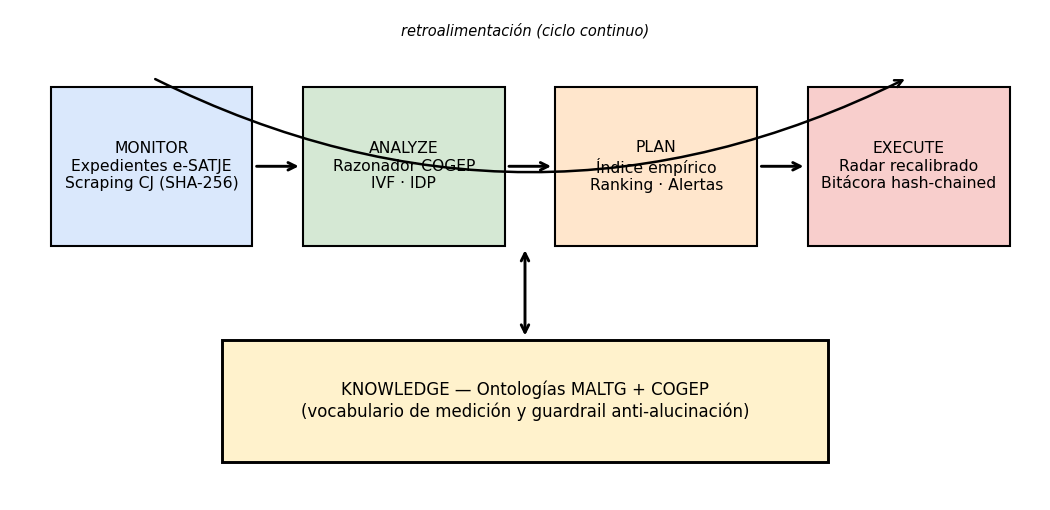
\includegraphics[width=0.95\textwidth]{Figuras/fig_mapek}
\caption{Arquitectura del ciclo adaptativo MAPE-K sobre las ontologías (Knowledge).}\label{fig:mapek}
\end{figure}

\section{Datos, materiales y recursos}
Corpus procesal: 47 causas públicas del portal SATJE (2022: 28; 2023: 8; 2024: 11), 12 provincias (Guayas 13, Pichincha 13, El Oro 4, Los Ríos 4, resto $\le$3), formato JSON con historial de actuaciones. Corpus documental: 15 corridas de captura con \textit{manifest} SHA-256. Conocimiento normativo: KB COGEP versionada. Flujos canónicos BPMN del e-SATJE. Infraestructura: FastAPI/Python 3.12 dockerizada, inferencia local y determinista.

\section{Variables, factores y escenarios de estudio}
\begin{table}[H]\centering\footnotesize
\caption{Variables del estudio y definición operacional.}\label{tab:vars}
\begin{tabular}{p{2.6cm}p{8.6cm}p{1.6cm}}\toprule
\textbf{Variable} & \textbf{Definición operacional} & \textbf{Rango} \\ \midrule
Salud procesal & Media de puntos por término evaluado (CUMPLE=100, ALERTA=60, INCUMPLE=0) & 0--100 \\
Índice empírico & Actos en plazo / actos evaluables (corpus completo) & 0--100 \\
IVF & $100\cdot$(actos no canónicos + faltantes)/(canónicos + no canónicos) & 0--100 \\
IDP & $\sum$ puntos por hallazgo de drift, acotada & 0--100 \\
Riesgo & $w_1(100-\text{salud}) + w_2\,\text{IVF} + w_3\,\text{IDP}$ & 0--100 \\
$\Psi(d)$ & $w_r\,\mathbb{1}[\text{root}\in R] + w_s\,|sub\cap R|/|sub|$ & 0--1 \\
F1 macro & Media armónica precision/recall por clase, promediada & 0--1 \\ \bottomrule
\end{tabular}\end{table}
Escenarios: \textbf{E1} medición empírica \textit{baseline}; \textbf{E2} variabilidad, deriva y alertas; \textbf{E3} cambio normativo con re-evaluación de impacto; \textbf{E4} validez del razonador contra \textit{gold standard}; \textbf{E5} ponderación experta y sensibilidad.

\section{Métodos y técnicas empleadas}
El Algoritmo~\ref{alg:razonador} formaliza el razonador; el Algoritmo~\ref{alg:drift} los detectores de deriva.
\begin{algorithm}[H]
\caption{Razonador simbólico de términos COGEP (cognitive digital shadow)}\label{alg:razonador}
\begin{algorithmic}[1]
\REQUIRE causa $c$ (actuaciones ordenadas), KB COGEP, calendario judicial $F$
\STATE $proc \leftarrow$ detectarProcedimiento($c$, KB) \COMMENT{por flujo BPMN o tipo de acción}
\FORALL{actuación $a \in c$}
  \STATE $acto(a) \leftarrow$ matchLéxico($a$, KB.actos) \COMMENT{vocabulario cerrado; sin match $\Rightarrow$ fuera de frontera}
\ENDFOR
\FORALL{regla $r \in$ KB.reglas con $proc \in r.procedimientos$}
  \STATE $r \leftarrow$ reglaVigente($r$, fecha del acto) \COMMENT{aplicación temporal de la norma (M3)}
  \STATE $d \leftarrow$ díasHábiles(fecha($r.desde$), fecha($r.hasta$), $F$) \COMMENT{Arts. 73/77 COGEP}
  \IF{$d \le r.termino$} \STATE veredicto $\leftarrow$ CUMPLE
  \ELSIF{$d \le r.termino \cdot \phi$} \STATE veredicto $\leftarrow$ ALERTA \COMMENT{$\phi$: factor configurable, def. 1.25}
  \ELSE \STATE veredicto $\leftarrow$ INCUMPLE \COMMENT{Art. 93 COGEP}
  \ENDIF
  \STATE emitir dictamen con cadena acto$\to$regla$\to$artículo + \texttt{contexto\_adaptacion}
\ENDFOR
\RETURN salud$(c)$ = media de puntos por término evaluado
\end{algorithmic}
\end{algorithm}
\begin{algorithm}[H]
\caption{Detección de deriva procesal (IDP) con criterio normativo primario}\label{alg:drift}
\begin{algorithmic}[1]
\REQUIRE traza de actuaciones de $c$, KB, configuración (puntos $p$, umbrales $k$, $g$)
\STATE \textbf{loops:} providencia repetida $\ge k$ veces $\Rightarrow$ hallazgo ($p_{loop}$)
\STATE \textbf{ping-pong:} patrón $A{\to}B{\to}A{\to}B$ en actos ontológicos $\Rightarrow$ hallazgo ($p_{pp}$)
\STATE \textbf{estancamiento legal:} término COGEP incumplido (del razonador) $\Rightarrow$ hallazgo ($p_{el}$, crítico)
\STATE \textbf{estancamiento referencial:} gap $> g$ días hábiles \textbf{sin} término aplicable $\Rightarrow$ hallazgo ($p_{er}$, rotulado sin fundamento normativo)
\STATE \textbf{retroceso:} acto de etapa $i$ tras actos de etapa $j>i$ (excluye notificaciones) $\Rightarrow$ hallazgo ($p_{re}$)
\RETURN IDP$(c) = \min(100, \sum p_i)$
\end{algorithmic}
\end{algorithm}
Complementariamente: análisis documental con protocolo de 4 fases y SHA-256; AHP con verificación CR~\cite{saaty1990}; Delphi/Likert con mediana normalizada; evaluación de clasificador contra \textit{gold standard} con doble anotación parcial ($\kappa$~\cite{cohen1960}); verificación ontológica (chequeos C1--C7, \textit{competency questions}, alineación LKIF-Core~\cite{casanovas2016}); sensibilidad por perturbación $\pm$10/20\%.

\section{Métricas y criterios de evaluación}
\begin{table}[H]\centering\footnotesize
\caption{Métricas y criterios de aceptación del artefacto.}\label{tab:criterios}
\begin{tabular}{p{4.2cm}p{4.6cm}p{4.6cm}}\toprule
\textbf{Dimensión} & \textbf{Métrica} & \textbf{Criterio de aceptación} \\ \midrule
Validez del mapeo IA & F1 macro vs gold standard & F1 $\ge 0.85$ (umbral configurable) \\
Objetividad de la tarea & $\kappa$ de Cohen (2 anotadores) & $\kappa \ge 0.70$ \\
Consistencia experta & CR de AHP & CR $< 0.10$ \\
Concordancia evaluadores & $\rho$ de Spearman (rúbrica) & $\rho \ge 0.70$ \\
Robustez & $\Delta$ score global ante $\pm$10\% & $\Delta < 5$; top-1 invariante ($\pm$20\%) \\
Adecuación ontológica & CQs; chequeos C1--C6 & 100\% CQs; 0 fallos críticos \\
No-alucinación & Salidas fuera de frontera & 0 respuestas inventadas \\ \bottomrule
\end{tabular}\end{table}

\section{Consideraciones éticas y de reproducibilidad}
Se usan exclusivamente causas de consulta pública; los indicadores se rotulan ``patrón de tramitación'' y toda salida porta el \textit{disclaimer} de no constituir asesoría jurídica. Reproducibilidad: evidencia congelada con SHA-256; \texttt{contexto\_adaptacion} (hashes de KB, calendario, configuración, versión del razonador) en cada resultado; bitácora \textit{append-only} encadenada por hash; sesión simulada con semilla fija (42) y marcado SIMULADO; artefacto dockerizado con datos JSON versionables. El Apéndice~\ref{ap:repro} detalla el protocolo completo de reproducción.

% ══════════════════════ CAPÍTULO 4 ══════════════════════
\chapter{Propuesta y resultados experimentales}
\section{Descripción general de la propuesta}
MALTG opera como ciclo MAPE-K sobre dos ontologías (Figura~\ref{fig:mapek}). \textbf{Monitor} observa el corpus de expedientes del e-SATJE y el ecosistema documental del Consejo de la Judicatura; \textbf{Analyze} aplica el razonador (Algoritmo~\ref{alg:razonador}) y los detectores (Algoritmo~\ref{alg:drift}); \textbf{Plan} agrega índice empírico, ranking de riesgo y alertas; \textbf{Execute} recalibra el radar de gobernanza y asienta la corrida en la bitácora. Las ecuaciones centrales son:
\begin{equation}
\Psi(d) = w_r\cdot\mathbb{1}[\text{root}_d\in R] + w_s\cdot\frac{|sub_d\cap R|}{|sub_d|},\qquad w_r+w_s=1
\end{equation}
\begin{equation}
riesgo(c) = w_1(100-salud_c) + w_2\,IVF_c + w_3\,IDP_c,\qquad
score_{LT} = (1-\lambda)\cdot declarado + \lambda\cdot I_{emp}
\end{equation}
donde $R$ es el conjunto de conceptos MALTG cubiertos por el SDT, $\lambda$ el peso empírico configurable e $I_{emp}$ el índice empírico global. La función $\Psi$ generaliza la \emph{hierarchical coverage function} publicada en~\cite{paccha2026info} (allí con pesos fijos 0.4/0.6): en esta tesis sus pesos se vuelven parámetros gobernados por AHP o por el panel de supuestos, cerrando la crítica de arbitrariedad. Análogamente, el radar de 10 dimensiones extiende el \textit{Bimodal Audit Method} y el GTI publicados en~\cite{paccha2026etcm}: donde BAM produce una clasificación binaria de cumplimiento por dominio (GTI=80.89 sobre la arquitectura de referencia, con TOGAF 91.7 como capa más madura y LegalTech 69.1 como brecha principal), el ciclo adaptativo introduce la dimensión temporal y empírica --- el cumplimiento deja de auditarse una vez y pasa a medirse continuamente.

\section{Componentes y funcionamiento del modelo}
El artefacto se organiza en 13 módulos navegables; los centrales para la experimentación son el radar de validación (10 dimensiones $\times$ $\Psi$), la \textit{cognitive digital shadow} COGEP, la capa adaptativa (supuestos mín--máx, calendario judicial, ranking, alertas, cambio normativo, muestra) y la validación experta (gold standard, AHP, Delphi, doble evaluación, verificación externa). La KB COGEP contiene 16 \textit{ActoProcesal}, 11 \textit{TerminoProcesal}, 7 \textit{Procedimiento} y 4 \textit{SujetoProcesal}, exportables a OWL con 7 \textit{object properties}.

\section{Implementación y configuración experimental}
Backend FastAPI (Python 3.12, $\sim$3\,500 LOC) con $\sim$65 \textit{endpoints}; frontend HTML/JS autocontenido; despliegue \texttt{docker compose} con \textit{hot-reload}. La configuración experimental completa se declara en la Tabla~\ref{tab:supuestos}: ningún parámetro de la simulación queda fuera del panel de supuestos, y cada cambio se valida contra sus límites en el servidor y se asienta en bitácora con hash.
\begin{table}[H]\centering\footnotesize
\caption{Supuestos del experimento: valores por defecto y límites admisibles (panel configurable).}\label{tab:supuestos}
\begin{tabular}{p{4.6cm}ccp{4.6cm}}\toprule
\textbf{Supuesto} & \textbf{Default} & \textbf{Rango} & \textbf{Rol} \\ \midrule
Peso ranking: salud & 0.50 & [0,1] & $w_1$ del score de riesgo \\
Peso ranking: variabilidad (IVF) & 0.25 & [0,1] & $w_2$ \\
Peso ranking: deriva (IDP) & 0.25 & [0,1] & $w_3$ \\
Peso empírico en el radar ($\lambda$) & 0.50 & [0,1] & Mezcla declarado/empírico \\
$\Psi$: peso del concepto raíz ($w_r$) & 0.40 & [0.1,0.9] & Justificable vía AHP \\
Puntos drift: loop / ping-pong & 20 / 15 & [0,50] & Aporte al IDP \\
Puntos drift: estanc. legal / referencial & 25 / 10 & [0,50] & Aporte al IDP \\
Puntos drift: retroceso & 20 & [0,50] & Aporte al IDP \\
Umbral loop $k$ & 3 & [2,10] & Repeticiones mínimas \\
Umbral gap referencial & 60 & [5,365] & Días hábiles \\
Factor ALERTA$\to$INCUMPLE ($\phi$) & 1.25 & [1.0,2.0] & Veredicto del razonador \\
Umbral de aceptación F1 & 0.85 & [0.5,1.0] & Aptitud del razonador \\ \bottomrule
\end{tabular}\end{table}

\section{Resultados experimentales}
\subsection{E1 --- Medición empírica del cumplimiento procesal (baseline)}
Sobre 47 causas (60 términos evaluables), el índice empírico global es \textbf{36.7/100} (22/60 actos en plazo), con salud media por causa de 44.4/100. La Tabla~\ref{tab:e1} y la Figura~\ref{fig:indiceproc} desglosan por procedimiento; la Figura~\ref{fig:dims} contrasta el score declarado de cada dimensión de gobernanza con el score del SDT tras el cierre adaptativo: la dimensión Legaltech pasa de 50.8 (declarado) a 43.8 con $\lambda=0.5$, y el score global del ecosistema queda en 25.1/100 frente a 73.9/100 de la ontología de referencia. \textbf{Hallazgo H-1:} la brecha declarado-vs-medido (48.8 puntos globales) es cuantificable y trazable; confirma H1/RQ1.
\begin{table}[H]\centering\footnotesize
\caption{E1 --- Cumplimiento por procedimiento (corpus SATJE, corte 2026-07).}\label{tab:e1}
\begin{tabular}{lcccccc}\toprule
\textbf{Procedimiento} & \textbf{N causas} & \textbf{Términos eval.} & \textbf{En plazo} & \textbf{Incumpl.} & \textbf{Índice} & \textbf{Salud media} \\ \midrule
SUMARIO   & 29 & 45 & 16 & 27 & 35.6 & 39.3 \\
MONITORIO & 17 & 15 & 6  & 9  & 40.0 & 55.6 \\
APELACIÓN & 1  & 0  & 0  & 0  & ---  & --- \\ \midrule
\textbf{Total} & \textbf{47} & \textbf{60} & \textbf{22} & \textbf{36} & \textbf{36.7} & \textbf{44.4} \\ \bottomrule
\end{tabular}\end{table}
\begin{figure}[H]\centering
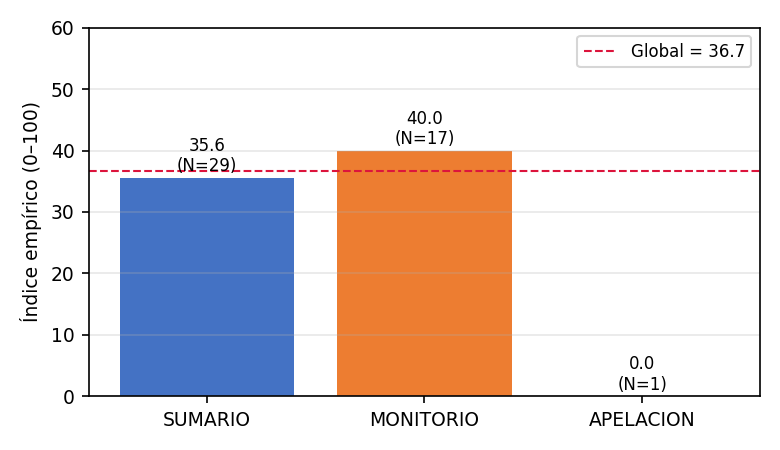
\includegraphics[width=0.62\textwidth]{Figuras/fig_indice_proc}
\caption{E1 --- Índice empírico por procedimiento; la línea discontinua marca el índice global (36.7).}\label{fig:indiceproc}
\end{figure}
\begin{figure}[H]\centering
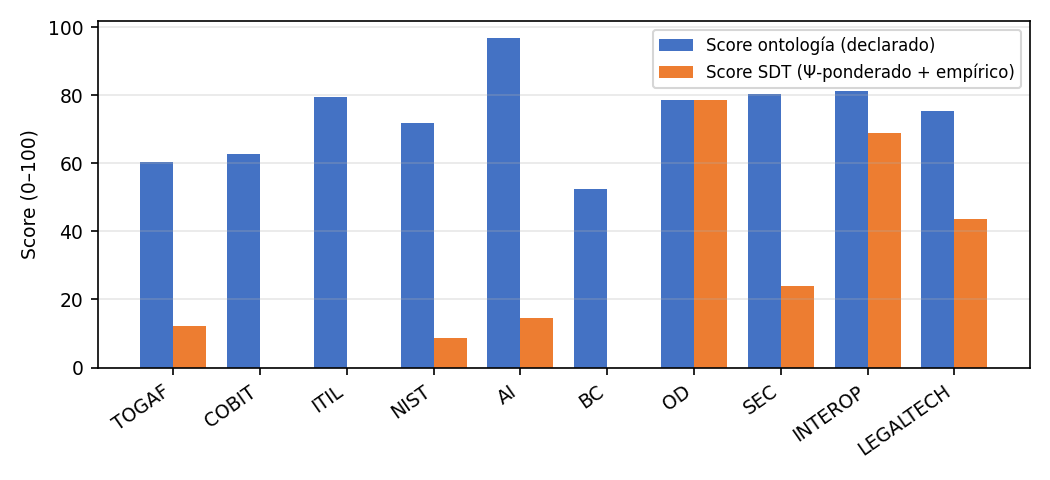
\includegraphics[width=0.95\textwidth]{Figuras/fig_dimensiones}
\caption{Score declarado (ontología) vs.\ score medido del SDT por dimensión de gobernanza, tras el cierre adaptativo ($\lambda=0.5$ en LEGALTECH).}\label{fig:dims}
\end{figure}

\subsection{E2 --- Variabilidad fáctica, deriva procesal y seguridad cognitiva}
La Figura~\ref{fig:ivfidp} muestra la dispersión IVF--IDP del corpus coloreada por salud procesal, y la Tabla~\ref{tab:top10} el \textit{top}-10 del ranking de riesgo con los pesos por defecto. \textbf{Hallazgo H-2:} existe un clúster de causas con salud 0, IVF $>$ 60 e IDP saturado (100) ---tramitación atípica con dilación normativamente fundada--- encabezado por la causa 09332202417826 (riesgo 96.9). El sistema de alertas produce 289 alertas: 36 críticas (término vencido, con artículo COGEP citado), 95 altas (patrón dilatorio) y 158 medias (actuaciones fuera de la frontera ontológica, derivadas a criterio humano). \textbf{Hallazgo H-3:} el conteo de ``fuera de frontera'' opera como métrica de no-alucinación: el sistema exhibe sus rechazos en lugar de aventurar clasificaciones (criterio 7 de la Tabla~\ref{tab:criterios} cumplido por construcción).
\begin{table}[H]\centering\footnotesize
\caption{E2 --- Top-10 del ranking de riesgo ($w_1{=}0.5, w_2{=}w_3{=}0.25$).}\label{tab:top10}
\begin{tabular}{clcccccc}\toprule
\# & \textbf{Causa} & \textbf{Proc.} & \textbf{Salud} & \textbf{IVF} & \textbf{IDP} & \textbf{Riesgo} \\ \midrule
1 & 09332202417826 & SUMARIO & 0.0 & 87.5 & 100 & 96.9 \\
2 & 17230202200143 & MONITORIO & 0.0 & 85.7 & 100 & 96.4 \\
3 & 12332202200022 & SUMARIO & 0.0 & 82.4 & 100 & 95.6 \\
4 & 12332202200023 & SUMARIO & 0.0 & 82.4 & 100 & 95.6 \\
5 & 13337202301582 & SUMARIO & 0.0 & 80.0 & 100 & 95.0 \\
6 & 07333202200092 & SUMARIO & 0.0 & 68.8 & 100 & 92.2 \\
7 & 12332202200024 & SUMARIO & 0.0 & 78.6 & 90 & 92.2 \\
8 & 09332202417790 & SUMARIO & 0.0 & 88.2 & 75 & 90.8 \\
9 & 09332202200107 & MONITORIO & 0.0 & 61.1 & 100 & 90.3 \\
10 & 17233202200296 & SUMARIO & 25.0 & 65.0 & 100 & 78.8 \\ \bottomrule
\end{tabular}\end{table}
\begin{figure}[H]\centering
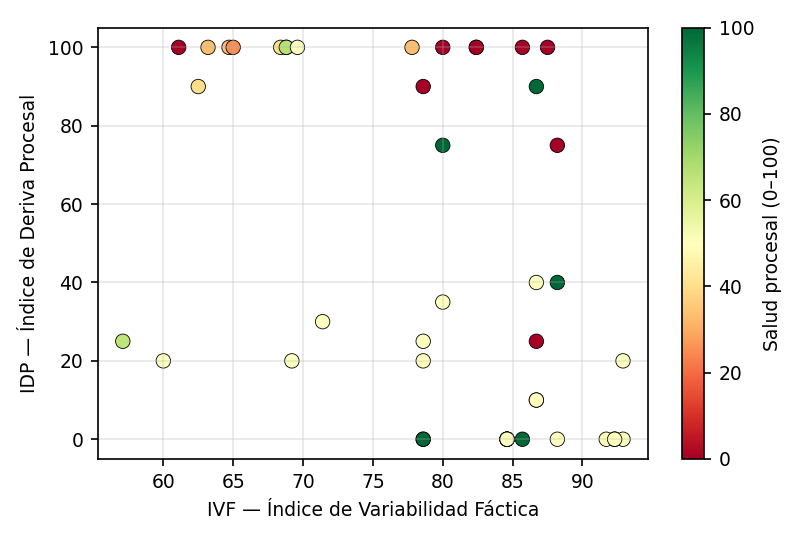
\includegraphics[width=0.72\textwidth]{Figuras/fig_ivf_idp}
\caption{E2 --- Dispersión IVF vs.\ IDP del corpus (color: salud procesal). El cuadrante superior derecho concentra la tramitación atípica y dilatoria.}\label{fig:ivfidp}
\end{figure}

\subsection{E3 --- Adaptación normativa con aplicación temporal}
Escenario controlado: reforma simulada de la regla \texttt{R\_CALIF} (calificación de la demanda), término $5\to3$ días hábiles con vigencia 2024-01-01 y fuente declarada como simulación. La cadena verificada fue: (i) la KB versionó la regla (v1.0$\to$v1.1) preservando el \textit{historial}; (ii) el razonador aplicó a cada acto la versión vigente a su fecha (aplicación temporal de la norma); (iii) la re-evaluación de impacto sobre el corpus identificó 3 causas evaluables para la regla y \textbf{1 cambio de dictamen} (CUMPLE$\to$INCUMPLE: 5 días computados frente al nuevo término de 3); (iv) el delta se propagó a ranking, alertas y radar en la misma corrida, con asiento en bitácora. \textbf{Hallazgo H-4:} el costo de evaluar el impacto de una reforma sobre todo el corpus es de una sola corrida ($<$5 s), habilitando el análisis normativo prospectivo (confirma H4/RQ4).

\subsection{E4 --- Validez del razonador contra gold standard}
El instrumento se demuestra extremo a extremo con la sesión simulada reproducible (semilla 42): 40 anotaciones de un anotador sintético que coincide $\sim$85\% con el sistema, 15 de un segundo anotador y evaluación automática. Resultados (Tabla~\ref{tab:e4}, Figura~\ref{fig:conf}): exactitud del mapeo 0.855, F1 macro 0.621 (\textit{precision} 0.578, \textit{recall} 0.693), $\kappa=0.833$ (acuerdo casi perfecto según~\cite{landis1977}) sobre 15 ítems comunes, y exactitud del veredicto 1.0 ($n=4$). \textbf{Hallazgo H-5:} el F1 macro penaliza correctamente las clases minoritarias donde el matching léxico falla (\texttt{act\_oposicion}, \texttt{act\_convocatoria}, \texttt{act\_embargo}: F1 = 0), mientras las clases frecuentes rinden alto (\texttt{act\_calificacion}: F1 = 1.0, $n{=}13$; \texttt{ninguno}: F1 = 0.889, $n{=}23$): la matriz de confusión orienta exactamente qué \textit{keywords} reforzar. Con el umbral de aceptación 0.85, el veredicto del instrumento es \textbf{no apto} ---resultado deliberadamente pedagógico que demuestra que el sistema no se auto-aprueba---. La sesión real con abogado anotador reemplaza estas cifras mediante la misma interfaz, y el \textit{chip} de validez de toda la aplicación se actualiza automáticamente.
\begin{table}[H]\centering\footnotesize
\caption{E4 --- Métricas por clase (sesión simulada, semilla 42; clases con $n>0$).}\label{tab:e4}
\begin{tabular}{lcccc}\toprule
\textbf{Clase (acto)} & \textbf{Precision} & \textbf{Recall} & \textbf{F1} & \textbf{n} \\ \midrule
act\_calificacion & 1.000 & 1.000 & 1.000 & 13 \\
ninguno (fuera de frontera) & 0.909 & 0.870 & 0.889 & 23 \\
act\_audiencia & 0.750 & 1.000 & 0.857 & 3 \\
act\_inadmision & 0.600 & 1.000 & 0.750 & 3 \\
act\_apelacion / act\_contestacion & 1.000 & 1.000 & 1.000 & 2+2 \\
act\_citacion & 0.600 & 0.750 & 0.667 & 4 \\
act\_recepcion & 0.500 & 1.000 & 0.667 & 1 \\
act\_oposicion / convocatoria / embargo & 0.000 & 0.000 & 0.000 & 2+1+1 \\ \midrule
\textbf{Macro} & \textbf{0.578} & \textbf{0.693} & \textbf{0.621} & \textbf{55} \\ \bottomrule
\end{tabular}\end{table}
\begin{figure}[H]\centering
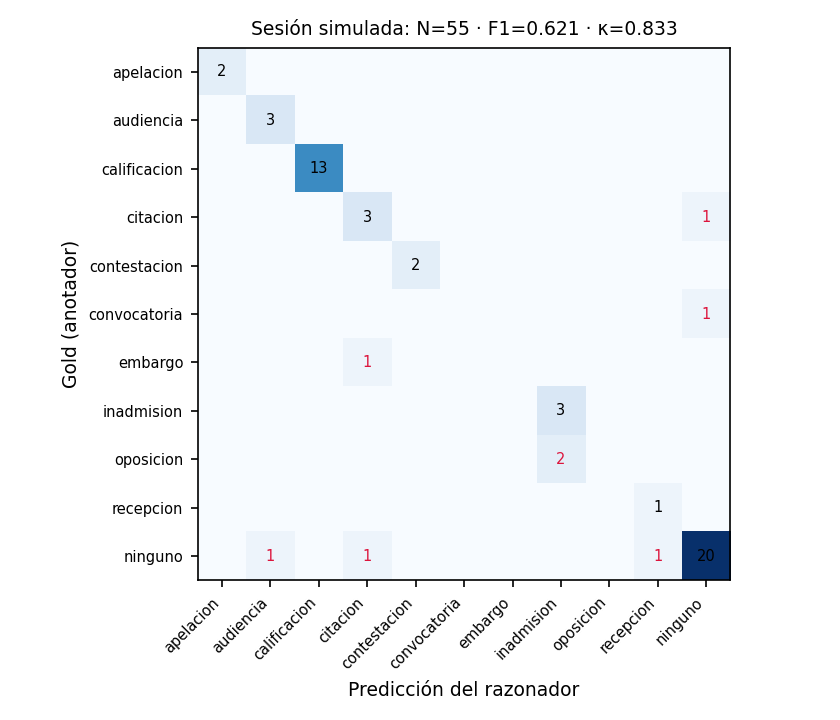
\includegraphics[width=0.8\textwidth]{Figuras/fig_confusion}
\caption{E4 --- Matriz de confusión gold vs.\ predicción (sesión simulada). La diagonal concentra los aciertos; las celdas rojas son el insumo del análisis de errores.}\label{fig:conf}
\end{figure}

\subsection{E5 --- Ponderación experta y análisis de sensibilidad}
El instrumento AHP (comparación raíz/subconceptos, escala Saaty, CR$\equiv$0 en matriz $2{\times}2$, agregación por media entre expertos) y el panel Delphi dimensional (importancia 1--9, mediana normalizada) alimentan pesos con procedencia declarada; en la corrida de instrumentación, la ponderación dimensional desplazó el score global de 23.4 a 26.2, evidenciando la respuesta del radar a los juicios expertos. La doble evaluación con rúbrica registró $\rho=0.718$ entre evaluadores de prueba y $\rho=0.884/0.840$ frente al sistema (valores demostrativos). El análisis de sensibilidad (Figura~\ref{fig:tornado}) perturbó $w_r\in\{0.32,\ldots,0.48\}$ ($\pm$20\%): el score global varía entre 24.6 y 25.5 (desviación máxima \textbf{0.5} puntos $<$ 5) y el \textit{top}-1 del ranking es invariante ante $\pm$20\% en $w_1,w_2,w_3$. \textbf{Hallazgo H-6:} las conclusiones del modelo no dependen del valor exacto de los pesos asumidos; el criterio de robustez de la Tabla~\ref{tab:criterios} se cumple.
\begin{figure}[H]\centering
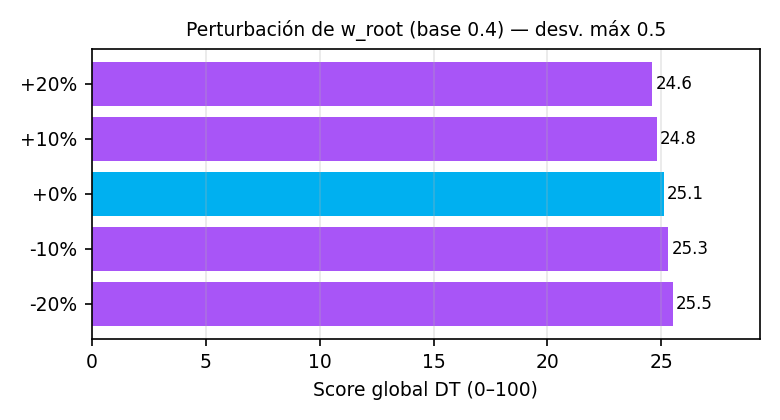
\includegraphics[width=0.62\textwidth]{Figuras/fig_tornado}
\caption{E5 --- Sensibilidad del score global ante la perturbación de $w_r$ ($\pm$10/20\%).}\label{fig:tornado}
\end{figure}

\subsection{Verificación ontológica}
La ontología COGEP exportada a OWL supera los chequeos estructurales C1--C6 (referencias íntegras de actos, reglas, procedimientos y sujetos; términos positivos con artículo; \textit{keywords} de matching) con única advertencia C7 (2 actos transversales fuera de etapas, justificados); las 10 \textit{competency questions} se responden en su totalidad con su consulta SPARQL equivalente documentada; y la alineación declarativa con LKIF-Core/LegalRuleML (6 correspondencias \textit{subClassOf}/\textit{closeMatch}) demuestra expresabilidad en los estándares del dominio~\cite{casanovas2016,suarez2015}. La verificación DL externa (HermiT/Protégé) y OOPS!~\cite{poveda2014} se asientan en el registro de verificación externa con el hash del OWL verificado.

\section{Análisis y discusión}
Tres hallazgos estructuran la discusión. \textbf{Primero}, la brecha declarado-vs-medido (73.9 vs.\ 25.1 global; 50.8 vs.\ 36.7 en la dimensión legaltech): un modelo estático jamás revelaría esta distancia, que es precisamente el objeto de la gobernanza adaptativa~\cite{janssen2016}. \textbf{Segundo}, el criterio normativo primario en la detección de deriva evita el falso positivo estadístico del \textit{process mining} convencional~\cite{bose2014}: un intervalo largo solo es estancamiento si viola un término del COGEP; lo demás se rotula referencial. \textbf{Tercero}, el \textit{guardrail} ontológico convierte la limitación del matching léxico en virtud metodológica: los rechazos son visibles (158 alertas ``fuera de frontera''), la validez es una cifra pública (chip F1) y el propio instrumento declaró \textit{no apto} al razonador en la sesión simulada ---el sistema no se auto-aprueba.

\section{Contribuciones científico-teóricas incorporadas en el artefacto}
Siguiendo la anatomía de una teoría de diseño de Gregor y Jones~\cite{gregor2007}, se explicita el contenido teórico que el artefacto encarna --- la respuesta a \emph{qué conocimiento nuevo queda en pie si se apaga el software}.

\textbf{(i) Constructos.} La tesis introduce y operacionaliza cinco constructos medibles, inexistentes como tales en la literatura previa: el \emph{índice empírico de cumplimiento procesal} ($I_{emp}$: proporción de términos legales satisfechos sobre el corpus, ancla empírica de la gobernanza); el \emph{Índice de Variabilidad Fáctica} (IVF: distancia entre el contexto fáctico de la tramitación y el flujo canónico normativo); el \emph{Índice de Deriva Procesal} (IDP: dilación fundada normativamente, no estadísticamente); la \emph{frontera ontológica} (conjunto de salidas admisibles de la IA, con su complemento observable ``fuera de frontera'' como métrica de no-alucinación); y el \emph{contexto de adaptación} (tupla de hashes que hace a cada resultado función explícita del conocimiento con que se produjo).

\textbf{(ii) Principios de forma y función.} Cinco principios de diseño, cada uno instanciado y verificable en la herramienta: \textbf{PD1 --- primacía normativa}: ningún indicador procesal se define estadísticamente si existe una regla jurídica aplicable (Algoritmo~\ref{alg:drift}, l.~3--4); \textbf{PD2 --- conocimiento como guardrail}: la misma ontología que define qué se mide define qué puede afirmar la IA (Algoritmo~\ref{alg:razonador}, l.~3); \textbf{PD3 --- adaptación trazable}: toda recalibración es una transacción con procedencia criptográfica (bitácora \textit{hash-chained} + \texttt{contexto\_adaptacion}); \textbf{PD4 --- validez pública}: el desempeño medido del componente de IA es un atributo visible de la interfaz (chip F1), no un dato de apéndice --- el sistema puede declararse a sí mismo \emph{no apto}; \textbf{PD5 --- supuestos acotados}: todo valor asumido es un parámetro declarado con rango admisible $[\min,\max]$, procedencia y asiento en bitácora --- la simulación no tiene parámetros ocultos.

\textbf{(iii) Proposiciones contrastables.} Las hipótesis H1--H4 (Tabla~\ref{tab:rq}) funcionan como proposiciones de la teoría: los resultados E1--E5 las corroboran en la instancia estudiada, y la teoría predice que cualquier instanciación del patrón (otra jurisdicción con términos procesales tasados, otro corpus de expedientes electrónicos, otras ontologías de dominio) exhibirá las mismas propiedades: brecha declarado-vs-medido cuantificable, dilación detectable con fundamento normativo, no-alucinación por construcción y reproducibilidad por procedencia.

\textbf{(iv) Mutabilidad del artefacto.} La teoría delimita qué puede cambiar sin romperse: la KB normativa (versionada con vigencias), el calendario, los pesos y umbrales (panel de supuestos), el clasificador providencia$\to$acto (sustituible por un extractor neuronal bajo el mismo guardrail y el mismo \textit{gold standard}) y el propio dominio (el patrón MAPE-K ontológicamente gobernado no contiene nada específicamente ecuatoriano salvo su \textit{Knowledge}).

\textbf{(v) Linaje teórico respecto de las publicaciones previas.} Cada contribución teórica es el refinamiento de un resultado publicado: $\Psi$ parametrizada refina la cobertura jerárquica de~\cite{paccha2026info}; el radar adaptativo refina BAM/GTI~\cite{paccha2026etcm}; la capa de fundamentos del SDT instancia~\cite{paccha2026silos}; las dimensiones del modelo instancian~\cite{paccha2026colim}; y la agenda completa responde a las brechas de la SLR~\cite{paccha2025slr}. La cadena publicación$\to$tesis es, en sí misma, una demostración del ciclo de rigor de DSR~\cite{hevner2004}.

\section{Amenazas a la validez}
\textbf{Constructo:} IVF/IDP son \textit{proxies}; se mitigó anclando el estancamiento al término legal y declarando los umbrales como supuestos configurables con rango. \textbf{Interna:} el cómputo de días hábiles depende del calendario configurado; feriados o suspensiones omitidos producen falsos INCUMPLE (mitigado con calendario editable, trazado y con 55 feriados 2022--2026 precargados). \textbf{Externa:} muestreo intencional (N=47, dominado por SUMARIO y MONITORIO): generalización analítica, no poblacional. \textbf{Conclusión:} las métricas E4/E5 provienen de la sesión simulada de instrumentación; el diseño obliga a reemplazarlas por las sesiones reales (el banner de datos simulados lo señala de forma permanente) antes de cualquier afirmación definitiva.

% ══════════════════════ CAPÍTULO 5 ══════════════════════
\chapter{Conclusiones y trabajo futuro}
\section{Aportes y contribuciones de la tesis}
\textbf{(RQ1)} El ciclo MAPE-K implementado recalibra el radar de 10 dimensiones desde la medición de 60 términos procesales reales, con cada recálculo trazado (H1 confirmada). \textbf{(RQ2)} El razonador produce dictámenes con cadena verificable acto$\to$regla$\to$artículo; la frontera ontológica elimina la alucinación por construcción y la instrumentación de validez (F1, $\kappa$, matriz de confusión) queda operativa y demostrada (H2: instrumentación confirmada; medición definitiva sujeta a la sesión real). \textbf{(RQ3)} Los detectores con criterio normativo identifican el clúster dilatorio con ranking robusto ante $\pm$20\% (H3 confirmada). \textbf{(RQ4)} Los metadatos de contexto y la bitácora \textit{hash-chained} hacen reproducible cada resultado histórico (H4 confirmada). Las contribuciones C1--C4 quedan materializadas en un artefacto público, dockerizado y auto-documentado, y su contenido teórico se explicita como teoría de diseño (constructos, principios PD1--PD5, proposiciones y mutabilidad) en la Sección~4.7, en continuidad con la trayectoria publicada P1--P5 (Tabla~\ref{tab:pubs}).
\section{Limitaciones del estudio}
(i) La validez definitiva del razonador requiere la sesión real de anotación; (ii) la muestra intencional limita la generalización estadística; (iii) el matching léxico no captura providencias semánticamente ambiguas (las clases con F1$=$0 de la Tabla~\ref{tab:e4} orientan la mejora); (iv) la verificación DL se ejecuta con herramientas externas; (v) el artefacto es una \textit{shadow}: la retroalimentación al e-SATJE excede el alcance institucional de una tesis.
\section{Líneas de trabajo futuro}
\textbf{F1} Cierre hacia \textit{digital twin} pleno (notificación de alertas al sistema real)~\cite{kritzinger2018,zheng2022}; \textbf{F2} ampliación muestral sistemática (N$\ge$100) con estadística por estrato; \textbf{F3} hibridación neurosimbólica: un LLM como extractor de candidatos bajo el mismo \textit{guardrail} y evaluado contra el mismo \textit{gold standard}~\cite{garcez2023}; \textbf{F4} formalización ejecutable en LegalRuleML y razonamiento DL integrado; \textbf{F5} AHP completo $9{\times}9$ multi-experto con agregación geométrica; \textbf{F6} estudio longitudinal del índice empírico como serie temporal de la salud procesal institucional.
\section{Consideraciones finales}
El resultado central es un cambio de categoría: del modelo de madurez que se responde con un cuestionario, al sistema de medición adaptativo que se responde con evidencia. En un dominio donde cada afirmación tiene consecuencias jurídicas, la combinación de ontologías como frontera, medición empírica como retroalimentación y trazabilidad criptográfica como memoria constituye el estándar mínimo exigible a la IA de gobernanza judicial.

% ══════════════════════ APÉNDICE ══════════════════════
\appendix
\chapter{Protocolo de reproducción de las experimentaciones}\label{ap:repro}
\section{Entorno}
\begin{enumerate}
\item Requisitos: Docker $\ge$ 24 y Docker Compose. Artefacto: repositorio del proyecto (backend FastAPI, frontend, datos en \texttt{env/data}).
\item Despliegue: \texttt{docker compose up} (imagen \texttt{python:3.12-slim}; puerto 8080; \textit{healthcheck} en \texttt{/api/health}).
\item Datos: 47 causas JSON en \texttt{/data/LegalCase}; KB en \texttt{/data/cogep\_kb.json}; calendario en \texttt{/data/feriados\_judiciales.json}; evidencia en \texttt{/data/evidence/<corrida>/manifest.json} (verificable con \texttt{GET /api/evidence/verify}).
\end{enumerate}
\section{Corridas por escenario}
\begin{table}[H]\centering\footnotesize
\caption{Endpoints de reproducción por escenario experimental.}\label{tab:repro}
\begin{tabular}{p{1.2cm}p{6.6cm}p{5.6cm}}\toprule
\textbf{Esc.} & \textbf{Comando (HTTP)} & \textbf{Salida esperada} \\ \midrule
E1 & \texttt{GET /api/cogep/salud-global} & \texttt{indice\_global=36.7}, 47 causas, 60 evaluables (Tabla~\ref{tab:e1}) \\
E2 & \texttt{GET /api/adaptativo/ranking} · \texttt{GET /api/adaptativo/alertas} & Tabla~\ref{tab:top10}; 289 alertas (36/95/158) \\
E3 & \texttt{POST /api/adaptativo/kb-cambio} (R\_CALIF, 3 días, 2024-01-01) · \texttt{GET /api/adaptativo/impacto} & 1/3 causas cambia CUMPLE$\to$INCUMPLE \\
E4 & \texttt{POST /api/experto/simulacion \{accion:crear\}} (semilla interna 42) & F1=0.621, $\kappa$=0.833, N=55 (Tabla~\ref{tab:e4}); limpiar con \texttt{\{accion:limpiar\}} \\
E5 & \texttt{POST /api/ahp} · \texttt{POST /api/experto/pesos-dimensiones} · \texttt{GET /api/sensibilidad} & Figura~\ref{fig:tornado}; estabilidad $\pm$10\% \\
Onto & \texttt{POST /api/cogep/owl/generar} · \texttt{GET /api/cogep/owl/verificacion} · \texttt{GET /api/cogep/cq} & C1--C6 OK, C7 advertencia; CQs 10/10 \\ \bottomrule
\end{tabular}\end{table}
\section{Trazabilidad}
Cada respuesta incluye \texttt{contexto\_adaptacion} con los hashes SHA-256 de la KB, el calendario, la configuración y la versión del razonador, más el \textit{timestamp} y el disparador. La bitácora (\texttt{GET /api/bitacora}) es \textit{append-only} con encadenamiento de hashes verificable (\texttt{cadena\_integra=true}). Para congelar los valores del documento: ejecutar E1--E5, exportar los JSON de respuesta y archivar junto a \texttt{salud\_global\_cache.json} y los \textit{manifests} de evidencia.

\bibliographystyle{ieeetr}
\bibliography{Bibliografia_MALTG}
\end{document}
